\documentclass[10pt]{article}
\usepackage[margin=0.8in]{geometry}
\usepackage{amsmath,amssymb,booktabs,tabularx,array,graphicx}
\usepackage[table]{xcolor}
\usepackage{float}
\usepackage{needspace}
\usepackage[T1]{fontenc}
\usepackage{lmodern}
\usepackage[hidelinks]{hyperref}
\title{Supplementary Methods: Shared LSTM Forecasts in MPC--DWA for UAV Path Planning among Dynamic Obstacles}
\author{}
\date{}
\begin{document}
\maketitle
\renewcommand{\thetable}{S\arabic{table}}
\renewcommand{\thefigure}{S\arabic{figure}}
\renewcommand{\theequation}{S\arabic{equation}}

\section*{S1. Development controller and trust-weight calibration}
This supplement documents the 3-s development configuration, Stage-1 trust-weight calibration and LSTM training (S1--S3); preserves the completed historical five-controller benchmark and earlier CV/Kalman studies (S4--S7); and reports the current 100-scene, seven-method exploratory evaluation (S8). Stage 1 comprised 4,320 development episodes and selected a trust-weight vector; these runs are separate from both the 7,500-run historical benchmark and the 2,100 planned exploratory episodes, and their selected weights were not applied to the historical benchmark. The historical benchmark used 1-s DWA screening and inherited weights listed with the development settings and identified explicitly in S4. Obstacle trajectories are exogenous: they are generated before a run and do not react to the UAV. The development and exploratory configurations use 3-s MPC and DWA horizons; in the shared-LSTM arm, the same time-aligned 30-step forecast reaches both layers. One-layer ablations send LSTM only to the named layer and use CV extrapolation in the other. DWA samples reachable controls and selects the command applied at the next 0.1-s update; MPC optimizes a 3-s control sequence and uses bounds from DWA's passing controls to constrain its first input. The three evidence sets are not pooled.

\subsection*{S1.1. MPC objective and first-control constraint}
The route term measures squared distance from each predicted position to the direct start-to-goal line. The complete objective and its geometric definitions are
\begin{equation}
\begin{aligned}
\mathbf{a}&=\mathbf{g}-\mathbf{s},\\
\eta_{\mathbf a}&=\mathbf a^{\mathsf T}\mathbf a+10^{-12}\,\mathrm m^2,\\
P_{\mathbf a}&=I_3-\frac{\mathbf a\mathbf a^{\mathsf T}}{\eta_{\mathbf a}},\\
\mathbf{e}_{t+k|t}^{\perp}&=P_{\mathbf a}(\mathbf{p}_{t+k|t}-\mathbf{s}),\\
J_{\mathrm{MPC}}={}&w_p\sum_{k=0}^{N-1}\|\mathbf{p}_{t+k|t}-\mathbf{g}\|_2^2\\
&+w_u\sum_{k=1}^{N}\|\mathbf{u}_{t+k|t}\|_2^2\\
&+w_f\|\mathbf{p}_{t+N|t}-\mathbf{g}\|_2^2\\
&+w_{\Delta u}\sum_{k=2}^{N}\|\mathbf{u}_{t+k|t}-\mathbf{u}_{t+k-1|t}\|_2^2 \\
&+w_r\sum_{k=1}^{N}\|\mathbf{e}_{t+k|t}^{\perp}\|_2^2 \\
&+\sum_{k=1}^{H_{\scriptstyle\mathrm{inj}}}\sum_{j=1}^{M}
\left[w_o\max(0,-\hat d_{j,k})^2+w_s\max(0,d_{\mathrm{soft}}-\hat d_{j,k})^2\right],\\
\text{subject to }\quad
&\mathbf{x}_{t|t}=\mathbf{x}_t,\\
&\mathbf{x}_{t+k|t}=f(\mathbf{x}_{t+k-1|t},\mathbf{u}_{t+k|t}),\quad k=1,\ldots,N,\\
&0\leq v_{c,t+k|t}\leq2.0~\mathrm{m\,s^{-1}},\\
&|\omega_{\theta,t+k|t}|\leq0.8~\mathrm{rad\,s^{-1}},\quad
|\omega_{\psi,t+k|t}|\leq0.8~\mathrm{rad\,s^{-1}},\quad k=1,\ldots,N.
\end{aligned}
\end{equation}
Here $\mathbf{x}_t=[\mathbf p_t^{\mathsf T},\theta_t,\psi_t,v_t]^{\mathsf T}$ is the current state in the implementation's position--pitch--yaw--speed order, and $f$ is the discrete vehicle update defined in the main text; the constraints initialize the prediction and propagate each planned state. The vectors $\mathbf s$ and $\mathbf g$ are the start and goal, and $\mathbf a=\mathbf g-\mathbf s$ is the start-to-goal route vector. The scalar $\eta_{\mathbf a}=\mathbf a^{\mathsf T}\mathbf a+10^{-12}\,\mathrm m^2$ is the squared route length with the implementation's numerical safeguard; $P_{\mathbf a}=I_3-\mathbf a\mathbf a^{\mathsf T}/\eta_{\mathbf a}$ defines the corresponding regularized cross-track operator. Thus $\mathbf e_{t+k|t}^{\perp}$ is the regularized cross-track residual of predicted position $\mathbf p_{t+k|t}$ from the direct route, and $I_3$ is the 3-D identity. The index $k$ denotes a prediction step, $N=30$ is the MPC horizon, and $\mathbf u_{t+k|t}$ is the three-component command planned at time $t$ for step $t+k$. The obstacle index is $j=1,\ldots,M$; $H_{\mathrm{inj}}=30$ is the number of forecast positions injected into MPC. The predicted signed clearance $\hat d_{j,k}$ is defined in the main text; $\hat d^{(b)}_{j,k}$ below is its candidate-specific counterpart. The soft margin $d_{\mathrm{soft}}=0.35$ m is the desired MPC safety margin. Thus the seven weights multiply, in order, stage goal error, control effort, terminal goal error, direct-route deviation, command variation, predicted overlap and sub-margin clearance.
The weights for stage position, control effort, terminal position, control smoothing, route deviation, obstacle overlap and the safety margin are 1, 10, 1, 50, 3, 20,000 and 12,000, respectively. The safety margin is 0.35 m. Main simulations use 30 prediction steps and a 0.1 s integration step. The code squares speed and angular-rate command values in their native units without cross-channel normalization, so this is a heuristic scalarization rather than a dimensionally homogeneous physical energy; the control weight supplies the numerical scale relative to position-based costs. In its soft penalty, MPC adds a $10^{-12}\,\mathrm m^2$ numerical smoothing term when evaluating distance; DWA gates and swept-collision checks use the exact norm. The route-weight ablation alone removes the direct-route preference; all primary results retain it.

When DWA retains candidates, their component-wise control extrema form the box for MPC's first input; the implementation expands each bound by 0.1 in its native command units before clipping to physical limits.
\begin{equation}
\begin{aligned}
\text{for }\mathcal A_t\ne\varnothing:\quad
\mathcal U_t&=\prod_{i=1}^{3}\left[
\max\!\left(u_i^{\min},\min_{b\in\mathcal A_{\scriptstyle t}}u_{b,i}-\delta\right),
\min\!\left(u_i^{\max},\max_{b\in\mathcal A_{\scriptstyle t}}u_{b,i}+\delta\right)\right],\qquad
\delta=0.1.
\end{aligned}
\end{equation}
Here $\mathcal A_t$ is the nonempty set of DWA candidates that pass the gates defined below, $u_{b,i}$ is component $i$ of candidate $b$, and $u_i^{\min}$ and $u_i^{\max}$ are the physical lower and upper limits for that component. The Cartesian product forms the three-dimensional control box $\mathcal U_t$. The implementation applies the same numerical expansion $\delta=0.1$ separately in each of the three control coordinates, then clips each bound to that coordinate's physical limits; the controls have different physical units, so this is a code-specific heuristic margin rather than a common dimensional distance. When $\mathcal A_t$ is empty, no extrema or envelope are formed; MPC uses its ordinary physical bounds. The box constrains MPC but does not certify every command inside it.
Only the first MPC control is constrained by this box. Let $\mathbf u_0=\mathrm{UPREV}$ denote the last control actually applied to the vehicle; the first rate bound therefore compares $\mathbf u_1$ with $\mathbf u_0$. The command components are speed $v_c$ and pitch/yaw rates $\omega_\theta,\omega_\psi$; their hard bounds are shown above. Component $i$ satisfies $|u_{k,i}-u_{k-1,i}|\leq a_i\Delta t$ for $k=1,\ldots,N$, where $\mathbf a_u=[a_1,a_2,a_3]^{\mathsf T}$ contains the speed, pitch-rate and yaw-rate acceleration limits. If no DWA candidate passes, the MPC solve uses its ordinary physical input bounds. Command speed, angular-rate and per-step rate-of-change limits remain active in either case; there are no separate hard state-box bounds. IPOPT uses at most 300 iterations and a stopping tolerance of 0.000001.

\subsection*{S1.2. Heuristic score, sampling and safety gates}
The four normalized heuristic-score components measure predicted clearance, goal progress, agreement with the preceding MPC reference, and command smoothness. Their definitions are
\begin{equation}
\begin{aligned}
d_{\min}^{\mathrm{MPC}}&=\min_{1\leq j\leq M,\,1\leq k\leq N}\hat d_{j,k},\\
d_0&=\|\mathbf p_{\mathrm{ref},1|t-1}-\mathbf g\|_2,\quad
d_N=\|\mathbf p_{\mathrm{ref},N|t-1}-\mathbf g\|_2,\\
\Delta_p&=\|\mathbf p_t-\mathbf p_{\mathrm{ref},1|t-1}\|_2,\qquad
\Delta\mathbf u_k=\mathbf u_k-\mathbf u_{k-1},\\
\operatorname{clip}_{[0,1]}(x)&=\max(0,\min(1,x)),\\
\tau_{\rm sa}&=\mathrm{clip}_{[0,1]}\!\left(\frac{d_{\min}^{\mathrm{MPC}}-d_{\mathrm{low}}}{d_{\mathrm{high}}-d_{\mathrm{low}}}\right),\\
\tau_g&=\begin{cases}1,&d_0<10^{-6}\,\mathrm m,\\
\mathrm{clip}_{[0,1]}(1-d_N/d_0),&\text{otherwise},\end{cases}\\
\tau_{\rm ref}&=\exp[-\alpha_T\Delta_p],\\
\tau_{\rm sm}&=\mathrm{clip}_{[0,1]}\!\left[1-\frac{1}{3(N-1)}\sum_{i=1}^{3}\right.\\
&\left.\qquad\sum_{k=2}^{N}\frac{|\Delta u_{k,i}|}{a_{u,i}\Delta t}\right],\\
\tau&=\sigma_s\tau_{\rm sa}+\sigma_g\tau_g\\
&\quad+\sigma_t\tau_{\rm ref}+\sigma_m\tau_{\rm sm},
&\qquad \sigma_s+\sigma_g+\sigma_t+\sigma_m=1,\\
\mathbf a_u&=[1,\ 0.5,\ 0.5]^{\mathsf T},\\
B&=\operatorname{round}[300(1+\alpha e^{-\beta\tau})],\\
B_g&=\operatorname{round}(B\tau),\quad B_e=B-B_g.
\end{aligned}
\end{equation}
Here $d_{\min}^{\mathrm{MPC}}$ is the smallest predicted surface clearance along the MPC reference available before DWA sampling: the initial MPC solution at startup and the shifted previous solution thereafter. The same aligned reference and its control sequence supply the goal-progress, mismatch and smoothness scores. $d_{\mathrm{low}}=1$ m and $d_{\mathrm{high}}=5$ m are the lower and upper clearance anchors for the safety-trust normalization. The reference runs from $\mathbf p_{\mathrm{ref},1|t-1}$ to $\mathbf p_{\mathrm{ref},N|t-1}$; $d_0=\|\mathbf p_{\mathrm{ref},1|t-1}-\mathbf g\|_2$ and $d_N=\|\mathbf p_{\mathrm{ref},N|t-1}-\mathbf g\|_2$. Thus $\tau_g$ measures the reference route's clipped fractional reduction in goal distance, not progress from the current measured position. The mismatch $\Delta_p=\|\mathbf p_t-\mathbf p_{\mathrm{ref},1|t-1}\|_2$ defines the reference-agreement score $\tau_{\rm ref}=\exp(-\alpha_T\Delta_p)$: a smaller mismatch gives a larger score. The index $k$ runs over the $N=30$ planned control steps, and $i$ indexes desired speed, pitch rate and yaw rate.

In the MATLAB implementation, the same reference-tracking score is named $\tau_t$; its subscript denotes tracking, not elapsed time.
\needspace{3\baselineskip}
The vector $\mathbf a_u=[1,0.5,0.5]^{\mathsf T}$ gives the componentwise acceleration limits for desired speed, pitch rate and yaw rate, with units m s$^{-2}$, rad s$^{-2}$ and rad s$^{-2}$, respectively; $\Delta t=0.1$ s is the control period. The subscript in $\sigma_t$ labels the reference-tracking component, not elapsed time. The four dimensionless components $\tau_{\rm sa}$, $\tau_g$, $\tau_{\rm ref}$ and $\tau_{\rm sm}$ quantify predicted safety, goal progress, reference agreement and command smoothness; their weighted sum is the heuristic sampling score $\tau$.
The score components are limited to the range from zero to one. The sampling rule divides the $B$ randomly generated candidates between $B_g$ MPC-guided actions and $B_e$ uniformly distributed exploratory actions. Guided controls are drawn within 0.35 per control component of the clipped MPC command and clipped to the dynamic window. The clipped MPC command is also added, yielding one extra candidate. Their union is the candidate-control set $\mathcal B_t$. The dimensionless budget-gain coefficient is $\alpha=1$, distinct from the reference-mismatch decay rate $\alpha_T$.
The four nonnegative trust coefficients were selected from a prespecified finite grid of six vectors using 48 development scenes and three matched sampling seeds. This Stage-1 design comprised $6\times5\times48\times3=4{,}320$ episodes, one for each candidate vector, integrated arm, scene and seed. The selection score gives equal weight to five trust-using integrated arms: CV-coupled MPC--DWA, LSTM to MPC only, LSTM to DWA only, shared LSTM, and latest-position hold. For each arm, collision-free arrival is the fraction of its 144 runs that reached the goal without swept contact; collisions and all non-arrivals remain failures. Stage 1 selected $[\sigma_s,\sigma_g,\sigma_t,\sigma_m]=[0.15,0.15,0.15,0.55]$, with an equal-arm macro-average of 0.8042. At this selected vector, the development rates were 0.8958 for shared LSTM, 0.7431 for CV-coupled MPC--DWA, 0.8194 for LSTM-to-MPC-only, 0.8958 for LSTM-to-DWA-only, and 0.6667 for latest-position hold. These rates and the macro-average are descriptive results from the same development scenes used for selection, not held-out comparisons or evidence of generalization. A recovery audit revalidated all 4,320 existing records and recomputed the selection without generating simulations. The current 100-scene evaluation uses the selected vector, while these development outcomes remain descriptive and do not validate its performance. The historical 7,500-run benchmark used its inherited vector $[0.35,0.30,0.15,0.20]$ and remains a separate 1-s DWA study (S4). The earlier 864-episode six-setting comparison used a different protocol and was not reused.

\noindent The reference-mismatch decay $\alpha_T=3\,\mathrm{m}^{-1}$ and budget sensitivity $\beta=3$ are fixed implementation settings; neither was selected by the 4,320 Stage-1 episodes. The planned 5,760-episode Stage-2 grid was not completed or independently verified, so it provides no basis for describing either setting as calibrated or Stage-2-selected. Stage-2 records and protocol are retained as historical audit material only and are excluded from the evidence used for the current paper's main conclusions. The score $\tau$ and its four component scores are dimensionless, $\alpha_T$ has units m$^{-1}$ because it multiplies the position mismatch $\Delta_p$ in metres, and $\beta$ is dimensionless.

The signed clearance for each sampled path and its minimum over all obstacles and forecast steps are defined below. A path is retained only if it passes the clearance, corridor and stopping-distance gates.
\begin{equation}
\begin{aligned}
H_D&=\left\lceil T_D/\Delta t\right\rceil=30,\qquad
H_{\mathrm{eff}}=\min(H_D,H_{\mathrm{inj}},N_{\mathrm{pred}})=30,\\
\hat d^{(b)}_{j,k}&=\|\mathbf p^{(b)}_{t+k|t}-\hat{\mathbf o}_{j,t+k|t}\|_2-r_j-r_u,\\
d_{\min}^{(b)}&=\min_{1\leq j\leq M,\,1\leq k\leq H_{\scriptstyle\mathrm{eff}}}\hat d^{(b)}_{j,k},\\
\mathcal C_b=1&\iff \forall k=1,\ldots,H_{\mathrm{eff}}:\quad
0.5\leq z^{(b)}_{t+k|t}\leq9.5~\mathrm m\ \text{and}\
|z^{(b)}_{t+k|t}-z_{\mathrm{nom},k}^{(b)}|\leq3~\mathrm m,\\
\mathcal A_t&=\left\{b\in\mathcal B_t:\ d_{\min}^{(b)}>0.25~\mathrm m,\quad
\mathcal C_b=1,\quad (v_{\mathrm{end}}^{(b)})^2\leq
2(1.0~\mathrm{m\,s^{-2}})d_{\min}^{(b)}\right\}.
\end{aligned}
\end{equation}
Here $T_D=3$ s is the DWA candidate-rollout duration, $H_D$ its number of simulated UAV states, $N_{\mathrm{pred}}=30$ the network-output length and $H_{\mathrm{inj}}=30$ the configured cap on usable forecast steps. Candidate $b$ has predicted centre $\mathbf p^{(b)}_{t+k|t}$; its third coordinate $z^{(b)}_{t+k|t}$ is altitude. Obstacle $j$ has predicted centre $\hat{\mathbf o}_{j,t+k|t}$ and radius $r_j$, while the UAV radius is $r_u$. Their surface clearance is $\hat d^{(b)}_{j,k}$ and its minimum is $d_{\min}^{(b)}$. The indicator $\mathcal C_b$ equals one only when every rollout point stays inside the absolute altitude band and within 3 m of $z_{\mathrm{nom},k}^{(b)}$, the altitude of the closest point on the finite start-to-goal segment to that predicted position; the segment projection is clipped to its endpoints. Finally, $v_{\mathrm{end}}^{(b)}$ is terminal candidate speed; its inequality is the stopping-distance gate using 1.0 m s$^{-2}$ available deceleration. The candidate contains 30 future UAV states, so its clearance gate compares all 30 time-aligned UAV--obstacle state pairs at 0.1-s intervals; it does not minimize relative distance continuously between two predicted states. The reported collision-free-arrival endpoint is stricter: it independently audits the saved true UAV and obstacle paths by continuous piecewise-linear closest approach between consecutive simulator states. The 30-step sequence also enters the MPC objective. The corridor condition applies to every DWA rollout point; the nominal altitude is taken from the direct start-to-goal line at the path's clamped along-route position. The reachable dynamic window is updated from the previous control using the acceleration bounds.

\noindent The 30-step DWA gate checks discrete, time-aligned states; the separate continuous piecewise-linear swept-path audit is an evaluation rule, not a continuous-time safety guarantee.

\Needspace{15\baselineskip}
\subsection*{S1.3. Candidate score}
The score-to-weight mapping and normalized weights are
\begin{equation}
\begin{aligned}
q&=[1+\exp(-8(\tau-0.5))]^{-1},\\
(w'_p,w'_h,w'_v,w'_o)&=(0.10+0.20q,\ 0.08+0.14q,\ 0.12(1+q),\ 0.45-0.25q),\\
w_i^{\mathrm{DWA}}&=\frac{w'_i}{\sum_{r\in\{p,h,v,o\}}w'_r}.
\end{aligned}
\end{equation}
The logistic map converts $\tau$ to $q$, which smoothly changes four unnormalized score coefficients $w'_p$, $w'_h$, $w'_v$ and $w'_o$. Dividing each by their sum gives $w_i^{\mathrm{DWA}}$ for position, heading, velocity and obstacle clearance, respectively; the summation index $r$ runs over those four components.
The candidate scores compare the 30-step DWA rollout endpoint with the endpoint of the current 30-step MPC reference, reward useful speed and obstacle clearance, and penalize vertical deviation. In the definitions below, $\mathbf p_{b,D}$ and $v_b$ are the DWA candidate endpoint and speed, whereas $\mathbf p_{\mathrm{MPC},N}$ and $v_{\mathrm{MPC}}$ are the final position and speed of the current MPC reference. The vectors $\mathbf h_b$ and $\mathbf h_{\mathrm{MPC}}$ are the corresponding unit heading vectors formed from terminal pitch and yaw. All component scores are dimensionless.
\begin{equation}
\begin{aligned}
S_{p,b}&=\left(1+\frac{\|\mathbf p_{b,D}-\mathbf p_{\mathrm{MPC},N}\|_2}{1\,\mathrm m}\right)^{-1}, &
S_{h,b}&=\tfrac12(1+\mathbf h_b^{\mathsf T}\mathbf h_{\mathrm{MPC}}),\\
S_{v,b}&=\tfrac12\left[\left(1+\frac{|v_b-v_{\mathrm{MPC}}|}{1\,\mathrm{m\,s^{-1}}}\right)^{-1}+\frac{v_b}{2\,\mathrm{m\,s^{-1}}}\right],\\
S_{o,b}&=\frac{\min(d_{\min}^{(b)},5\,\mathrm m)}{5\,\mathrm m}, &
S_{z,b}&=\left(1+\frac{\max_{1\leq k\leq H_{\scriptstyle D}}|z_{b,k}-z_{\mathrm{nom},k}|}{1\,\mathrm m}\right)^{-1},\\
S_b&=w_p^{\mathrm{DWA}}S_{p,b}+w_h^{\mathrm{DWA}}S_{h,b}+w_v^{\mathrm{DWA}}S_{v,b}+w_o^{\mathrm{DWA}}S_{o,b}+w_zS_{z,b}.
\end{aligned}
\end{equation}
Here $S_{p,b}$, $S_{h,b}$, $S_{v,b}$, $S_{o,b}$ and $S_{z,b}$ are the position-agreement, heading-agreement, velocity, obstacle-clearance and vertical-corridor scores of candidate $b$. The value $z_{b,k}$ is its altitude at rollout step $k$, and $z_{\mathrm{nom},k}$ is the corresponding direct-route altitude. Their weighted total is $S_b$. The planner selects the retained candidate with the largest total score. The fixed coefficient is $w_z=0.25$; it is added after the four normalized weights and is not renormalized with them.

\subsection*{S1.4. Executed cycle and fallback}
The implemented top-to-bottom cycle is:
\begin{enumerate}
\item Read the current UAV state and the latest 10 obstacle observations.
\item Predict 30 future obstacle offsets with the causal LSTM; each offset is relative to the latest observed centre and is added directly, not cumulatively.
\item At startup, solve MPC from the current state with this forecast to initialize the reference route and control sequence, then compute the first trust score. At later updates, shift the preceding MPC solution forward before computing trust.
\item Align the MPC sequence and DWA rollouts over steps 1--30 of the same forecast; update the heuristic score using the available MPC reference and its first-point mismatch with the current position.
\item Sample score-guided DWA controls, roll each out for 3 s (30 steps at 0.1 s), and test those UAV states against all 30 forecast positions before applying the corridor and braking gates and scoring retained candidates.
\item If the normal safe set is nonempty, form its expanded first-control box and retain the top-scoring DWA command. Trigger lateral recentering when the selected rollout's minimum predicted clearance exceeds 1.0 m and the UAV's current horizontal cross-track offset from the start--goal line exceeds 0.5 m. Set yaw rate to 0.8 times the wrapped heading error toward the goal, clipped to the physical yaw-rate limit. Recompute the rollout and reapply the normal clearance, corridor and braking gates; use the adjusted command only if all gates pass, otherwise revert to the original screened sample.
\item If the normal safe set is empty, augment the reachable samples with low-speed controls at the lower edge of the dynamic window, a reachable pitch-rate command toward level flight, and bounded yaw-rate choices. Roll out every emergency candidate against the same forecast.
\item Retain an emergency candidate only when its predicted surface clearance is strictly positive, the full rollout remains within the flight corridor, and terminal speed satisfies the configured stopping-distance condition. Rank retained emergency candidates by predicted clearance, breaking ties toward lower terminal speed.
\item Recompute and re-screen the final emergency command against all three emergency conditions. If no candidate passes, mark the trial as having no feasible emergency action and terminate before issuing an unchecked command. This fail-closed simulator branch records planning infeasibility; it does not model instantaneous physical braking.
\item Re-solve MPC from the current state with the current forecast. Use the normal safe-set box only when the normal safe set is nonempty.
\item Execute the screened DWA or emergency command for 0.1 s; update state and observation history, and repeat.
\end{enumerate}
The emergency branch differs from the normal 0.25-m candidate gate: it permits smaller positive clearance when the predicted surfaces remain separated and the stopping-distance condition passes. The planner rechecks the exact selected command before execution. A trial also ends after at most 650 state updates, equivalent to 65 s. Goal arrival and an infeasible emergency-action stop terminate execution early; a detected collision is logged but does not itself stop the simulator. For the Stage-1 development episodes, goal arrival required final distance within the configured goal tolerance and no swept-path contact. The historical five-controller results retain the endpoint definition and audit used in their original run bundle.

\begin{center}
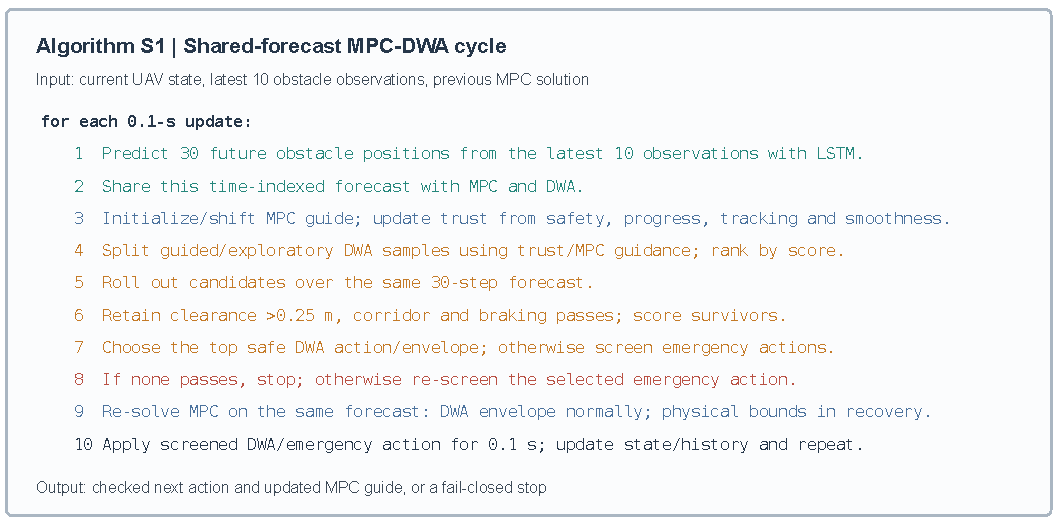
\includegraphics[width=0.98\linewidth]{figures/shared_forecast_pseudocode_algorithm_s1.pdf}
\end{center}

\section*{S2. LSTM training and prediction evaluation}
At each 0.1-s planning cycle, the predictor maps the latest 10 observations for each obstacle to 30 three-dimensional future offsets. Every offset is anchored independently to the latest observed centre; it is not added to the preceding forecast. Samples are separated by 0.1 s, so the first and last observations are 0.9 s apart. An observation contains position, velocity and heading encoded by its sine and cosine. In clean-observation evaluation, velocity and heading are simulator-provided obstacle states; heading is obstacle yaw, distinct from UAV yaw. In the separate noisy-input diagnostic, velocity is recomputed from perturbed positions while heading is unchanged. Table~\ref{tab:training} separates the network architecture from the data split and optimizer settings so the complete training configuration is easy to reproduce.

The training set contains synthetic trajectories from eight motion families. The split is made by trajectory, so no trajectory appears in both training and validation. Training inputs include current and one-step-delayed histories; a noisy view adds independent 0.03-m position noise while future targets remain clean and anchored to the noisy last observation. For noisy views, velocity is recomputed from perturbed positions, whereas simulator-generated heading remains unchanged. Normalization uses training trajectories only. Validation trajectories support model selection and early stopping; the independent open-loop probe is reported below.

\begin{table}[!htbp]
\centering
\caption{LSTM architecture and training configuration.}
\label{tab:training}
\small
\renewcommand{\arraystretch}{1.10}
\begin{tabularx}{\linewidth}{@{}>{\raggedright\arraybackslash}p{0.30\linewidth}X>{\raggedright\arraybackslash}p{0.23\linewidth}@{}}
\toprule
Parameter & Setting & Unit or definition \\
\midrule
\multicolumn{3}{@{}l}{\textit{Input and network}}\\
Input history & 10 observations; first-to-last span 0.9 s & 0.1-s interval \\
Input channels & Position, velocity, cosine heading, sine heading & 8 values per observation \\
LSTM layer & 96 hidden units; use final sequence output & 96 units \\
Dropout & 0.2 & Fraction \\
Fully connected layer & 96 units followed by ReLU & 96 units \\
Regression output & 90 displacement values & 30 steps $\times$ 3 axes \\
Forecast output & 30 offsets, each relative to the latest observed position & 3 s \\
\addlinespace[2pt]
\multicolumn{3}{@{}l}{\textit{Data and optimization}}\\
Synthetic training set & 800 trajectories from eight motion families & Generated trajectories \\
Trajectory split & 640 training; 160 validation & No shared trajectories \\
Noisy-history augmentation & Independent 0.03-m position noise; clean future targets & Training input \\
Optimizer & Adam; learning rate 0.001; batch size 128 & Per training run \\
Training limit & 180 epochs; validation every 50 iterations & Maximum \\
Regularization & L2 coefficient 0.0001; gradient threshold 1 & As implemented \\
Early stopping & Patience 12; retain best validation-loss model & Validation set \\
Random seed & 20260905 & Training-data setup \\
\bottomrule
\end{tabularx}
\end{table}

Validation trajectories are separate from training trajectories and support model selection and early stopping. A separate open-loop probe evaluates 12 independently generated synthetic compound switchback trajectories, with 14 forecast windows per trajectory. Each track combines repeated stop--go motion with piecewise turn-rate reversals; the compound test trajectories are held out from training. In each forecast window, ADE is the average three-dimensional centre-position error over the 30 predicted steps and FDE is the average error at the final step. Mean ADE/FDE are 0.626/1.254 m for LSTM, 0.865/1.544 m for constant velocity, 0.864/1.506 m for Kalman and 1.033/1.974 m for static positions. Paired trajectory-cluster bootstrap intervals for LSTM minus constant velocity are -0.259 to -0.218 m (ADE) and -0.350 to -0.228 m (FDE); for LSTM minus Kalman they are -0.275 to -0.201 m (ADE) and -0.331 to -0.173 m (FDE). The 20,000 bootstrap replicates resample the 12 trajectories, retaining all windows and paired method outcomes for each selected trajectory. These open-loop metrics quantify position-prediction accuracy; closed-loop planning performance is evaluated separately in S4.

Online ADE and FDE summarize diagnostic runs retained in the run-level CSV. Goal arrival is the primary closed-loop outcome; held-out switchback prediction results are available in the supplementary CSV records.

\section*{S3. Development simulation settings}
Tables~\ref{tab:scene-settings} and~\ref{tab:planner-settings} give the 3-s configuration used for Stage-1 development and the current seven-method evaluation. In this configuration, the network returns 30 positions over 3 s, DWA checks each reachable 3-s candidate rollout against positions 1--30, and MPC optimizes a 3-s route using the same time-aligned positions. A selected DWA command is applied for one 0.1-s update. The historical five-controller benchmark used 1-s DWA screening and is reported separately in S4.

\begin{table}[!htbp]
\centering
\caption{Workspace, vehicle and timing settings for the separate 3-s development configuration.}
\label{tab:scene-settings}
\small
\renewcommand{\arraystretch}{1.10}
\begin{tabularx}{\linewidth}{@{}>{\raggedright\arraybackslash}p{0.18\linewidth}Xr>{\raggedright\arraybackslash}p{0.20\linewidth}@{}}
\toprule
Group & Parameter & Value & Unit or definition \\
\midrule
\multicolumn{4}{@{}l}{\textit{Workspace}}\\
Scene & Workspace dimensions & $20\times20\times10$ & m (x, y, z) \\
Scene & UAV start & $(1,1,1)$ & m \\
Scene & Goal & $(18,18,8)$ & m \\
Flight envelope & Altitude band & $0.5$--$9.5$ & m (z-axis) \\
\addlinespace[2pt]
\multicolumn{4}{@{}l}{\textit{Vehicle model}}\\
Vehicle & Effective radius & 0.3 & m \\
Vehicle & Maximum speed & 2.0 & m s$^{-1}$ \\
Vehicle & Maximum pitch and yaw rates & 0.8 & rad s$^{-1}$ \\
Vehicle & Maximum linear acceleration & 1.0 & m s$^{-2}$ \\
Vehicle & Maximum pitch and yaw acceleration & 0.5 & rad s$^{-2}$ \\
\addlinespace[2pt]
\multicolumn{4}{@{}l}{\textit{Simulation time}}\\
Integration & State-update interval & 0.1 & s \\
Vehicle response & Speed-response time constant & 0.5 & s \\
Trial & Maximum duration & 650 updates & 65 s \\
\bottomrule
\end{tabularx}
\end{table}

\begin{table}[!htbp]
\centering
\caption{MPC and DWA parameters for the separate 3-s development configuration; the historical 1-s benchmark weights are identified separately.}
\label{tab:planner-settings}
\small
\renewcommand{\arraystretch}{1.10}
\begin{tabularx}{\linewidth}{@{}>{\raggedright\arraybackslash}p{0.16\linewidth}X>{\raggedright\arraybackslash}p{0.29\linewidth}@{}}
\toprule
Planner & Parameter & Value and definition \\
\midrule
\multicolumn{3}{@{}l}{\textit{Prediction and planning horizons}}\\
MPC & Route horizon & 30 steps (3 s) \\
DWA & Candidate rollout & 30 steps (3 s); selected command applied for one 0.1-s update \\
DWA & Forecast available / used by screening & All 30 predicted positions, time-aligned to the 3-s rollout \\
\addlinespace[2pt]
\multicolumn{3}{@{}l}{\textit{MPC objective and solver}}\\
MPC & Objective weights & $w_p,w_u,w_f,w_{\Delta u},w_r,w_o,w_s = 1,10,1,50,3,20{,}000,12{,}000$; in the S1.1 objective order \\
MPC & Soft safety margin & $d_{\mathrm{soft}}=0.35$ m \\
IPOPT & Iteration cap; stopping tolerance & 300; $10^{-6}$ \\
\addlinespace[2pt]
\multicolumn{3}{@{}l}{\textit{DWA sampling and score}}\\
DWA & Base sample budget & $N_{\mathrm{base}}=300$ candidates \\
DWA & Adaptive stochastic sample budget & $\operatorname{round}[300(1+\alpha e^{-\beta\tau})]$ with fixed $\alpha=1$; fraction $\tau$ guided, plus the clipped MPC command \\
DWA & Guided sampling half-width & $0.35$ in each native control unit; clipped to the dynamic window \\
DWA & Stage-1 development trust-score weights & $[0.15,0.15,0.15,0.55]$; equal-arm development rate 0.8042 \\
DWA & Historical benchmark trust-score weights (S4) & $[0.35,0.30,0.15,0.20]$; inherited, not tuned on the 500 scenes \\
DWA & Safety-trust normalization anchors & $d_{\mathrm{low}}=1$ m; $d_{\mathrm{high}}=5$ m \\
DWA & Reference-mismatch decay, $\alpha_T$ & $3$ m$^{-1}$ in Stage 1 and the historical benchmark \\
DWA & Budget sensitivity, $\beta$ & $3$ in Stage 1 and the historical benchmark \\
DWA & Logistic weight mapping & Dimensionless slope 8; dimensionless midpoint 0.5 (fixed implementation heuristics) \\
DWA & Candidate rejection and braking gate & Clearance $>0.25$ m; deceleration $1.0$ m s$^{-2}$ \\
DWA & Adaptive score-weight ranges & Position 0.10--0.30; heading 0.08--0.22; velocity base 0.12; obstacle 0.20--0.45 \\
DWA & Vertical-corridor score coefficient & $w_z=0.25$, additive and unnormalized (fixed implementation heuristic) \\
\bottomrule
\end{tabularx}
\end{table}

The historical five-controller scene bank was generated by \texttt{generate\_random\_eval\_scenarios} with master seed 20261015; scene seeds increase by one from 20261015 to 20261514. Each scene contains 3--8 obstacles, with each obstacle independently assigned one of seven motion families at equal probability: straight, turn, sinusoidal speed, acceleration, hover--go, zigzag or waypoint following. The manifest records each scene seed, obstacle count and assigned family. Obstacle radii are uniform on 1.0--1.8 m. Initial centres are placed 2--5 m to alternating sides of the start--goal diagonal, at stations formed from evenly spaced values between 3.8 and 14.6 m plus Gaussian jitter with a standard deviation (SD) of 0.25 m, clipped to 3.2--15.2 m; initial height is uniform on 2.2--8.0 m. Initial speed is uniform on 0.8--1.6 m s$^{-1}$, vertical speed is Gaussian with mean 0 and SD 0.03 m s$^{-1}$, and heading is set to either diagonal direction with Gaussian noise (SD 0.15 rad). Maneuver parameters are sampled within the ranges in the accompanying \texttt{scene\_generation\_specification.md}; the exact generator, manifest and historical per-run records accompany this supplement. The 48 development scenes used for Stage 1 were a separate scene set.

The trust score weights safety, goal progress, reference tracking (current-position mismatch to the one-step-old MPC reference) and command smoothness. High trust concentrates fewer samples near the clipped MPC command; low trust increases full-window exploration. The command is added once, and all candidates pass the same corridor and clearance checks. The $0.35$ guided-sampling half-width, logistic slope $8$, midpoint $0.5$ and vertical-score coefficient $w_z=0.25$ are fixed implementation heuristics, held constant in every integrated arm that uses them and not selected using held-out outcomes. The sampling half-width is applied in each control's native units ($\mathrm{m\,s^{-1}}$ for speed and $\mathrm{rad\,s^{-1}}$ for pitch and yaw rates) before clipping to the dynamic window; slope and midpoint are dimensionless. The additive $w_z$ term is distinct from the four trust weights and is not renormalized with them.

The historical two-method forecast-sharing runs used Windows 64-bit, MATLAB R2025a and CasADi 3.8.0 with the 1-s DWA rollout. Timing begins before obstacle prediction and ends after DWA screening, the MPC solve, state advancement and post-step logging; one-time solver setup is excluded. Table~\ref{tab:runtime} summarizes both the mean and median over timed steps. Each method had 1,500 timed runs. The mean step times differ by 0.07 ms in this environment. These descriptive local measurements are specific to this 1-s historical implementation and do not characterize the 3-s development configuration.

\begin{table}[ht]
\centering
\caption{Historical descriptive computation time in the two-method, 1-s DWA forecast-sharing evaluation. Step time covers prediction, planning, state advancement and logging; initialization is excluded.}
\label{tab:runtime}
\small
\renewcommand{\arraystretch}{1.12}
\begin{tabular}{@{}lrrrr@{}}
\toprule
Method & Attempts & Timed runs & Mean (ms/step) & Median (ms/step) \\
\midrule
DWA-only LSTM & 1500 & 1500 & 100.23 & 95.9 \\
Shared LSTM & 1500 & 1500 & 100.30 & 95.7 \\
\bottomrule
\end{tabular}
\end{table}

\section*{S4. Controller definitions and historical comparisons}
\subsection*{S4.1. Methods in the completed five-controller comparison}
The historical comparison comprised a latest-position-hold MPC--DWA reconstruction, standalone DWA + LSTM, standalone MPC + LSTM, integrated MPC--DWA with LSTM supplied only to DWA, and integrated MPC--DWA with the same LSTM forecast supplied to both layers. All five methods used the same 500 obstacle scenes and three matched sampling seeds. The latest-position reconstruction holds obstacle positions at their most recent observations in both MPC and DWA; it is a project-local implementation, not an exact reproduction of the cited MPC--DWA algorithm or its reported experiments.

The 3,000 shared-versus-DWA-only episodes are the corresponding two-arm records within this 7,500-run five-controller benchmark; they are not an additional set of simulation episodes.

Standalone DWA receives the causal LSTM forecast and samples a fixed grid over dynamically reachable speed, pitch-rate and yaw-rate commands. It scores 1-s rollouts without an MPC route, trust score or MPC-guided samples, then screens retained actions with clearance, corridor and braking checks. Standalone MPC receives the same type of LSTM forecast and optimizes the 30-step route objective, but directly applies its first command without DWA sampling or action screening; obstacle safety remains a soft objective penalty. In the integrated DWA-only condition, MPC holds latest observed obstacle positions while DWA uses LSTM forecasts. In the shared condition, both layers use the same time-aligned LSTM sequence. DWA screens its first 10 steps (1 s), whereas MPC uses all 30 steps (3 s). The shared-versus-DWA-only contrast therefore isolates forecast access by MPC within the tested integrated implementation; the independent controllers provide contextual, non-matched comparisons.

\subsection*{S4.2. Historical forecast-sharing comparison (1-s DWA rollout)}
The earlier forecast-sharing comparison used the same 500 independently generated mixed-motion 3D scenes (scenario master seed 20261015) and three matched sampling seeds per scene, for 1,500 runs in each integrated condition. Its 500-scene target followed a paired normal-approximation calculation based on the earlier 48-scene estimate (2.08 percentage points; scene-level SD, 15.99 percentage points), targeting 80\% power at a two-sided 5\% level. The trained predictor, vehicle model, planner objective, safety checks, sampler and stopping rules were fixed. The predictor returned the same 30-step (3-s) LSTM sequence in both conditions. DWA screened each 10-step (1-s) reachable action against forecast steps 1--10; MPC planned for 30 steps and, in the shared arm, used the full sequence. In the DWA-only arm MPC instead held obstacles at their latest observed positions. This contrast isolates MPC's access to the learned forecast. It differs from the 3-s development configuration described in S1--S3. The historical 48-scene experiment used a different DWA horizon and is reported separately. All scenes and attempts are included; the frozen design and analysis rule are in the earlier confirmatory protocol.

These earlier runs used clean, current-time simulator obstacle positions: observation noise and delay were both set to zero. Noisy and delayed histories were used in training augmentation and the separate S5 sensing diagnostic. The executed settings are documented in \url{confirmatory_protocol_clarification.md}. The endpoint was arrival within 0.5 m without collision, checked by closest approach along piecewise-linear motion between states. Runs not terminated earlier were classified as maximum-step non-arrivals after 650 updates (65 s). The paired contrast is shared LSTM minus DWA-only LSTM. We resampled the 500 complete scenes, retaining all three matched seeds and both methods, for 20,000 bootstrap replicates (MATLAB Twister seed 20261015). The prespecified criterion was a 95\% interval entirely above zero; intervals for secondary outcomes are unadjusted.

\begin{table}[H]
\centering
\caption{Historical mutually exclusive run outcomes (1,500 runs per method). Categories are assigned in order: safe arrival, any collision, collision-free infeasible stop, collision-free solver-only failure, then maximum-step non-arrival. Each column sums to 1,500.}
\label{tab:confirmatory_outcomes}
\small
\renewcommand{\arraystretch}{1.2}
\setlength{\tabcolsep}{6pt}
\begin{tabularx}{\linewidth}{@{}>{\raggedright\arraybackslash}X>{\centering\arraybackslash}p{0.28\linewidth}>{\centering\arraybackslash}p{0.28\linewidth}@{}}
\toprule
Outcome & \shortstack{Shared forecast\\(MPC and DWA)} & \shortstack{DWA-only forecast\\(DWA receives it)} \\
\midrule
\rowcolor{blue!8}
\textbf{Reached goal without collision, runs (\%)} & \textbf{936/1,500 (62.4\%)} & \textbf{836/1,500 (55.7\%)} \\
Collision recorded & 0 & 2 \\
No collision; infeasible-action stop & 366 & 453 \\
No collision/stop; solver-only failure & 0 & 0 \\
No collision/stop/solver; 650-step non-arrival & 198 & 209 \\
\bottomrule
\end{tabularx}
\end{table}

Two shared-arm runs recorded an MPC solve failure before later ending in the infeasible-stop category; the exclusive priority above prevents double counting. The complete event flags and the derived accounting are supplied in \url{five_method_run_audit.csv} and \url{five_method_terminal_outcomes.csv}.

\noindent\textbf{Historical result.} Sharing produced 100 more collision-free goal arrivals (936/1,500, 62.4\%, versus 836/1,500, 55.7\%; paired difference +6.7 percentage points, 95\% scene-cluster CI +4.2 to +9.2). It favored sharing in 72 scenes, favored DWA-only in 24, and tied in 404 (three seeds per scene).

The run-level minimum surface clearance averaged 1.245 $\pm$ 1.085 m with sharing and 1.187 $\pm$ 1.046 m with DWA-only prediction; the paired difference was +0.058 m (95\% scene-cluster CI +0.027 to +0.090; unadjusted secondary interval).

Distance travelled per run averaged 21.144 m with sharing and 19.743 m with DWA-only prediction; the paired difference was +1.401 m (95\% scene-cluster bootstrap CI +0.931 to +1.906; unadjusted secondary interval). This average includes successful and incomplete runs, so it combines route geometry with distance travelled before termination and is not interpreted as the cost of a detour.

The earlier 48-scene, six-forecast-setting experiment is reported separately because it used a different DWA rollout.

\subsection*{S4.3. Historical five-controller architecture comparison}
The integrated controllers in this 7,500-run benchmark used inherited trust weights $[0.35,0.30,0.15,0.20]$. The later Stage-1 development selection $[0.15,0.15,0.15,0.55]$ was not applied to these runs.
This earlier comparison's latest-position MPC--DWA, standalone DWA and standalone MPC arms reused the exact 500 scenes, obstacle tracks, plant settings and sampling seeds 1--3 from its confirmatory bundle. The coupled MPC--DWA arms and standalone DWA used 1-s DWA rollouts; MPC retained a 30-step horizon. The two standalone arms were regenerated in a versioned fairness rerun: standalone DWA used the integrated planner's strictly positive emergency-clearance rule, while its 0.25-m normal gate and all corridor and braking checks were unchanged; standalone MPC code and parameters were unchanged. The four LSTM-guided arms use the same frozen predictor; the latest-position baseline does not call it. Together the five arms contain 7,500 trials, 1,500 per controller.

The historical trust weights and the later Stage-1 development selection are distinct, as specified in S1.2. The earlier v08 standalone-DWA record reports 1,146/1,500 collision-free arrivals (76.4\%) with no collision runs; the versioned emergency-screen rerun used here reports 1,236/1,500 (82.4\%). These results come from distinct implementations and are retained separately, not pooled or substituted for one another. Parameters were not tuned on these evaluation outcomes.

Analysis resampled all three paired seeds within each of the 500 scenes for 20,000 scene-cluster bootstrap replicates. The shared-minus-latest-position contrast was frozen before the direct baseline run, and the shared-minus-DWA-only interval remains the original confirmatory contrast in that earlier protocol. Standalone-controller intervals are secondary and unadjusted for multiplicity. For the secondary \texttt{MedianPlanningStep\_ms} contrast, each scene contributes the median of its three run-level mean step times, and the reported point estimate is the mean paired difference across 500 scenes; this estimand differs from the descriptive method-level median over all 1,500 run-level mean step times in Table~\ref{tab:five-controller-summary}. These five-controller results are separate from the 3-s development configuration.

\begin{table}[H]
\centering
\caption{Earlier five matched controllers evaluated on 500 scenes with three seeds per scene. Collision-free arrival was the principal outcome within that comparison; mean minimum clearance is calculated per run from continuous swept paths. Planning time is descriptive and is not used to rank architectures because timing boundaries differ.}
\label{tab:five-controller-summary}
\small
\renewcommand{\arraystretch}{1.14}
\setlength{\tabcolsep}{4pt}
\begin{tabularx}{\linewidth}{@{}>{\raggedright\arraybackslash}X>{\centering\arraybackslash}p{0.22\linewidth}>{\centering\arraybackslash}p{0.15\linewidth}>{\centering\arraybackslash}p{0.15\linewidth}>{\centering\arraybackslash}p{0.16\linewidth}@{}}
\toprule
Controller & Collision-free goal arrival & Collision runs & Mean minimum gap (m) & Median step time (ms) \\
\midrule
MPC--DWA, latest-position-hold & 33/1,500 (2.2\%) & 624 (41.6\%) & 0.532 & 79.5 \\
Standalone DWA + LSTM & 1,236/1,500 (82.4\%) & 0 (0\%) & 1.515 & 5.9 \\
Standalone MPC + LSTM & 1,428/1,500 (95.2\%) & 36 (2.4\%) & 0.674 & 29.7 \\
Integrated MPC--DWA, DWA-only LSTM & 836/1,500 (55.7\%) & 2 (0.13\%) & 1.187 & 95.9 \\
Integrated MPC--DWA, shared LSTM & 936/1,500 (62.4\%) & 0 (0\%) & 1.245 & 95.7 \\
\bottomrule
\end{tabularx}
\end{table}

\begin{table}[H]
\centering
\caption{Exhaustive mutually exclusive terminal accounting for the five-controller comparison. Priority is safe arrival, any collision, collision-free infeasible-action stop, collision-free solver-failure termination, then collision-free 650-step non-arrival. Every row sums to 1,500.}
\label{tab:terminal-accounting}
\scriptsize
\renewcommand{\arraystretch}{1.12}
\setlength{\tabcolsep}{3.5pt}
\begin{tabularx}{\linewidth}{@{}>{\raggedright\arraybackslash}Xrrrrr@{}}
\toprule
Controller & Safe & Collision & Infeasible & Solver & 650-step \\
\midrule
MPC--DWA, latest-position-hold & 33 & 624 & 143 & 0 & 700 \\
Standalone DWA + LSTM & 1,236 & 0 & 264 & 0 & 0 \\
Standalone MPC + LSTM & 1,428 & 36 & 0 & 9 & 27 \\
Integrated MPC--DWA, DWA-only LSTM & 836 & 2 & 453 & 0 & 209 \\
Integrated MPC--DWA, shared LSTM & 936 & 0 & 366 & 0 & 198 \\
\bottomrule
\end{tabularx}
\end{table}

The accounting is derived from the saved run flags without rerunning the simulator and is archived in \url{five_method_terminal_outcomes.csv}. Collision is assigned before other failure flags because collision-free arrival is the primary endpoint; an integrated run can record an MPC solve failure and later stop infeasibly, so event totals outside this table may overlap.

Shared LSTM produced 903 more collision-free arrivals than latest-position MPC--DWA (936/1,500 versus 33/1,500), a paired increase of +60.2 percentage points (95\% scene-cluster CI +56.2 to +64.2). Collision incidence fell from 624/1,500 (41.6\%) to zero; the paired collision-rate difference was -41.6 points (95\% CI -45.5 to -37.5). Mean swept minimum clearance increased by 0.712 m (95\% CI +0.643 to +0.784). Descriptive median planning-time values were 79.5 ms for latest-position MPC--DWA and 95.7 ms for shared LSTM; the timing boundaries differed, so these values are not interpreted as a comparative efficiency effect. These results quantify historical outcomes for the reconstructed coupled architecture.

The shared controller's collision-free arrival was lower than standalone DWA by 20.0 percentage points (95\% paired scene-cluster CI, -24.8 to -15.1) and lower than standalone MPC by 32.8 points (-37.1 to -28.5). Standalone MPC reached the goal more often but had 36 swept-collision runs; shared LSTM had no collisions and a larger mean minimum gap. Standalone DWA also had no collisions, a larger mean minimum gap and higher arrival. The shared method is therefore the best tested coupled MPC--DWA variant, whereas standalone MPC has the highest overall arrival rate.

\section*{S5. Single-scene sensing-pressure check}
The sensing diagnostic evaluates one repeated-encounter scene with three matched seeds under four conditions: clean observations, 0.05-m position noise, one-step observation delay, and their combination. Obstacle paths and controller settings are fixed; these runs are separate from the 500-scene comparison in S4. In noisy conditions, noise affects positions only, velocity is recomputed from noisy positions, and heading $\psi$ remains the simulator-provided value, corresponding to an ideal heading observation. Table~\ref{tab:sensing} reports terminal outcomes, sampled clearance and forecast error. These four conditions are descriptive diagnostics of this single scene, not population-level or full-state sensor-noise robustness evidence.

\begin{table}[ht]
\centering
\caption{Shared-LSTM outcomes under four sensing conditions in one repeated-encounter scene. Each condition has three matched seeds. Clearance is the per-run minimum sampled at 0.1-s post-action states; ADE and FDE are the mean and standard deviation across seeds. Terminal counts and metric summaries are descriptive, not population estimates.}
\label{tab:sensing}
\footnotesize
\renewcommand{\arraystretch}{1.12}
\setlength{\tabcolsep}{3.5pt}
\begin{tabularx}{\linewidth}{@{}>{\raggedright\arraybackslash}Xrrrr>{\raggedright\arraybackslash}p{0.31\linewidth}@{}}
\toprule
Condition & \shortstack{Goals\\($n/3$)} & \shortstack{Collision\\runs ($n/3$)} & \shortstack{Infeasible\\stops ($n/3$)} & \shortstack{Clearance\\mean $\pm$ SD (m)} & \shortstack{ADE / FDE\\mean $\pm$ SD (m)} \\
\midrule
Clean & 0/3 & 0/3 & 3/3 & $0.924\pm0.674$ & $0.560\pm0.027\,/\,1.302\pm0.035$ \\
0.05-m position noise & 0/3 & 0/3 & 3/3 & $1.142\pm0.340$ & $0.667\pm0.019\,/\,1.480\pm0.036$ \\
One-step observation delay & 0/3 & 0/3 & 3/3 & $1.388\pm0.005$ & $0.610\pm0.000\,/\,1.397\pm0.000$ \\
Noise and delay & 0/3 & 0/3 & 3/3 & $1.023\pm0.422$ & $0.697\pm0.018\,/\,1.523\pm0.048$ \\
\bottomrule
\end{tabularx}
\end{table}

All 12 shared-LSTM runs ended in a fail-closed stop before reaching the goal; none recorded a collision. Under this obstacle trajectory, the planner found no feasible emergency action. Clearance and ADE/FDE are descriptive means and standard deviations across three seeds. The four-method summary is in \url{sensing_summary_revised.csv}; run-level records are in \url{sensing_revised.csv}.

\section*{S6. Earlier baseline comparisons retained separately}
Earlier baseline experiments compare static-position, constant-velocity (CV) and Kalman forecasts; their original figures and analysis records are retained in this section. Because these studies used different scenes and a different DWA action-rollout setting, they are reported separately from the historical 500-scene estimate and the current seven-method exploratory evaluation.

\subsection*{S6.1. Early 16-scene baseline pilot}
This historical pilot used four fixed scenes and 12 random scenes, each with three matched seeds; it is retained separately from the Stage-1 development calibration, the historical 500-scene benchmark and the current seven-method exploratory evaluation. In the fixed suite, goal arrivals were 10/12 for static positions, 9/12 for CV, 9/12 for Kalman and 12/12 for shared LSTM. In the random suite, arrivals were 26/36, 33/36, 33/36 and 36/36, respectively. The scene-cluster estimate for the random-suite shared-LSTM minus CV difference was +8.3 percentage points (95\% CI, 0.0 to 25.0), spanning zero. The earlier four-panel results figure is retained in Fig.~\ref{fig:legacy36}; its panels include random-scene success and clearance, forecast error and a single-scene interface/horizon ablation.

\begin{figure}[htbp]
\centering
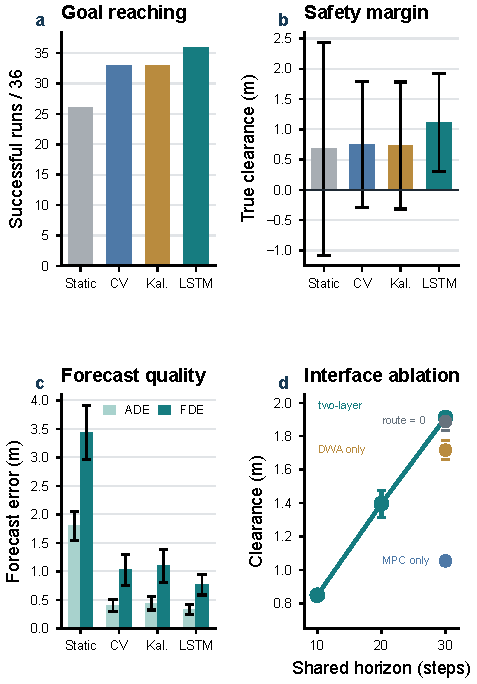
\includegraphics[width=0.85\linewidth]{figures/historical_36run_results.pdf}
\caption{Retained historical results figure from the earlier random-scene comparison (36 runs per method). It shows Static, CV, Kalman and shared LSTM, with separate forecast-error and single-scene interface/horizon panels. This pilot is reported separately and not pooled with the historical 500-scene benchmark or the seven-method exploratory evaluation.}
\label{fig:legacy36}
\end{figure}

\subsection*{S6.2. Earlier 48-scene, six-setting comparison}
The subsequent historical benchmark tested Static, CV, Kalman, MPC-only LSTM, DWA-only LSTM and shared LSTM in 48 scenes with three matched seeds per setting (144 runs per method; 864 attempts). Table~\ref{tab:historical48} reports method-level goal and failure outcomes; Fig.~\ref{fig:historical48} shows scene-cluster intervals and paired contrasts. The shared-LSTM versus CV contrast was the prespecified primary comparison in that study: 125/144 goal arrivals (86.8\%) versus 103/144 (71.5\%), a paired difference of +15.28 percentage points (95\% scene-cluster bootstrap CI, +6.25 to +25.69). The shared-versus-DWA-only difference was +2.08 percentage points (95\% CI, -1.39 to +6.94). Its DWA rollout differed from the 1-s rollout in the historical five-controller benchmark and the 3-s development configuration, so these estimates remain separate historical evidence.

\begin{table}[htbp]
\centering
\caption{Run-level outcomes in the earlier 48-scene six-setting comparison, with 144 attempts per method. Clearance is the mean $\pm$ standard deviation of each run's minimum. Collision, infeasible-stop and solver-failure counts are separately audited flags and may co-occur.}
\label{tab:historical48}
\footnotesize
\renewcommand{\arraystretch}{1.14}
\setlength{\tabcolsep}{3.5pt}
\begin{tabularx}{\linewidth}{@{}l r r r r >{\raggedleft\arraybackslash}X@{}}
\toprule
Method & Goals, $n/144$ (\%) & Collisions & Infeasible stops & Solver failures & Minimum clearance, mean $\pm$ SD (m) \\
\midrule
Static & 97/144 (67.4\%) & 24 & 44 & 0 & $1.038\pm1.121$ \\
CV & 103/144 (71.5\%) & 0 & 39 & 0 & $1.400\pm1.105$ \\
Kalman & 106/144 (73.6\%) & 0 & 36 & 1 & $1.335\pm1.079$ \\
MPC-only LSTM & 109/144 (75.7\%) & 23 & 34 & 0 & $1.035\pm1.095$ \\
DWA-only LSTM & 122/144 (84.7\%) & 0 & 22 & 0 & $1.465\pm1.029$ \\
Shared LSTM & 125/144 (86.8\%) & 0 & 19 & 0 & $1.425\pm0.980$ \\
\bottomrule
\end{tabularx}
\end{table}

Figure~\ref{fig:historical48} displays all six goal-arrival rates and the paired shared-LSTM contrasts. The CV contrast was prespecified in that benchmark; the remaining paired intervals are secondary and unadjusted. The complete run audit, scene-cluster outcomes, bootstrap contrasts, scenario manifest and protocol are retained in the separate historical 48-scene folder and the reproducibility archive.

\begin{figure}[htbp]
\centering
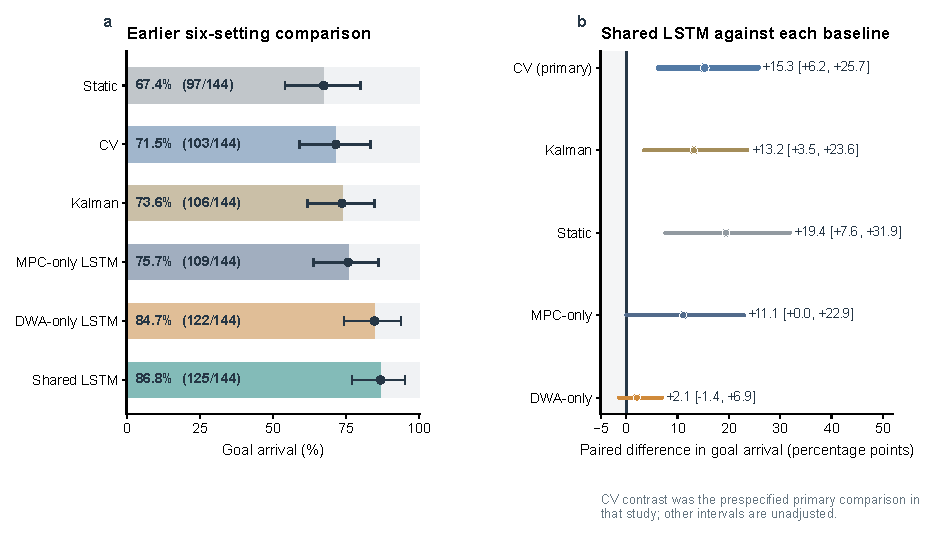
\includegraphics[width=\linewidth]{figures/historical_48scene_baselines.pdf}
\caption{Earlier six-setting comparison across 48 scenes. (a) Goal-arrival rates, with 95\% scene-cluster intervals and counts. (b) Paired success-rate differences (shared LSTM minus each baseline); the vertical line marks zero. The CV contrast was prespecified in that study; other intervals are unadjusted. These estimates are separate from the historical 500-scene benchmark and the current seven-method exploratory evaluation.}
\label{fig:historical48}
\end{figure}

The former main-text scene-2 route comparison is also retained as a historical illustration. It compares CV, Kalman, DWA-only LSTM and shared LSTM on the same prescribed obstacle tracks; these paths are separate from the new standalone-controller evaluation.
\begin{figure}[htbp]
\centering
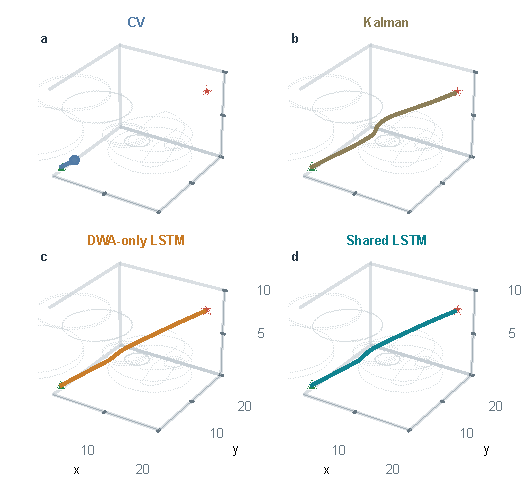
\includegraphics[width=0.78\linewidth]{figures/historical_scene2_four_controller_routes.pdf}
\caption{Historical four-method 3-D route example from scene 2 and DWA sampling seed 1. Panels (a)--(d) show CV, Kalman, DWA-only LSTM and shared LSTM under the same prescribed obstacle tracks. The green triangle marks the start, the red star the goal, and the open circle CV's recorded early-stop endpoint. In this example, CV stopped before the goal; the other three methods reached the goal, and all four routes were collision-free under the swept-path test. Each route contains only its saved states through the recorded terminal point; none is extended or interpolated. Obstacle tracks show scene context and are not time-aligned with route durations. This single historical example illustrates route geometry, not aggregate performance, and is reported separately from the historical five-controller benchmark and current seven-method evaluation.}
\label{fig:historical-scene2}
\end{figure}

\section*{S7. Representative routes from the earlier five-controller comparison}
Fig.~\ref{fig:primaryroutes} shows the historical scene 404, seed 2 example for the reconstructed latest-position MPC--DWA baseline and four LSTM-guided controllers under identical obstacle tracks. The reconstructed baseline collides at step 224 (minimum swept clearance, $-0.0603$ m). Standalone DWA + LSTM stops after 20 steps, 22.06 m from the goal, following an infeasible action set. Standalone MPC + LSTM collides at step 262; although its final state is 0.49 m from the goal, its minimum swept clearance is $-0.236$ m. In the integrated DWA-only-LSTM run, no safe candidate or feasible emergency action remains after 220 steps, leaving the UAV 16.23 m from the goal. Only integrated shared LSTM reaches without collision, after 253 steps with 0.583 m minimum swept clearance. Each overlaid route contains only recorded states through its terminal step. In the figure, $\times$ indicates a swept collision somewhere along a run, not its terminal point; square and circle markers denote a stop and collision-free arrival, respectively. This selected scene is illustrative; aggregate outcomes are tabulated separately in Table~\ref{tab:five-controller-summary}. It is one case from the historical five-controller comparison, not an estimate of overall performance.

\begin{figure}[htbp]
\centering
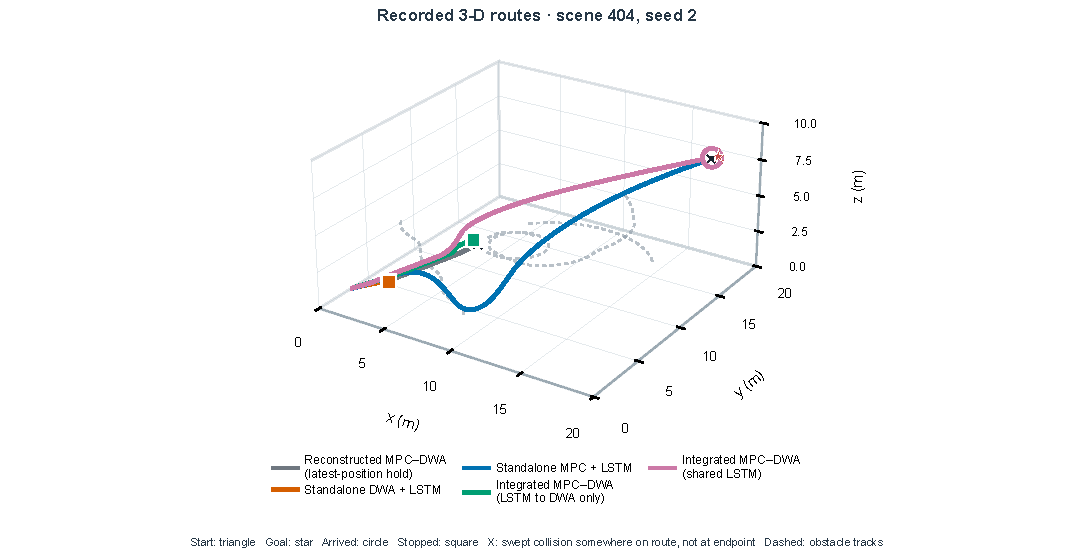
\includegraphics[width=0.99\linewidth]{figures/route_comparison.pdf}
\caption{Historical five-controller 3-D route overlay from scene 404, seed 2 in a 20 m $\times$ 20 m $\times$ 10 m workspace. The five overlaid routes are reconstructed MPC--DWA with latest-position-hold (collision, step 224), standalone DWA + LSTM (stopped, step 20), standalone MPC + LSTM (collision, step 262), integrated MPC--DWA with LSTM supplied only to DWA (stopped, step 220), and integrated MPC--DWA with shared LSTM (collision-free goal arrival, step 253). Each trajectory ends at its logged terminal state. The triangle and star mark the common start and goal; squares denote stops, circles denote collision-free arrival, and $\times$ denotes a swept collision somewhere along that run, not at the marker. Dashed lines show the in-workspace portions of the same three obstacle tracks. This route-only illustration has no aggregate-rate panel; aggregate outcomes are tabulated separately in Table~\ref{tab:five-controller-summary}.}
\label{fig:primaryroutes}
\end{figure}

\section*{S8. Seven-method exploratory evaluation}
\subsection*{S8.1. Frozen design and outcome definitions}
This limited-scope evaluation compares seven matched controller arms on 100 newly generated, unique-content-hashed scenes, with sampling seeds 1--3 shared across all methods (300 episodes per arm; 2,100 planned episodes total). The arms are standalone DWA with CV prediction, standalone MPC with CV prediction, coupled MPC--DWA with CV in both layers, coupled MPC--DWA with LSTM supplied to MPC only, coupled MPC--DWA with LSTM supplied to DWA only, coupled MPC--DWA with the same LSTM forecast supplied to both layers, and a project-local latest-position-hold MPC--DWA reconstruction. The last arm is an architectural reconstruction, not an exact reproduction of the cited method. All arms use 0.1-s updates, a 30-step (3-s) MPC horizon and, unlike the historical five-controller benchmark, a 30-step DWA screening horizon. The trust vector was selected in the separate 4,320-episode Stage-1 development sweep; $\alpha_T=3\,\mathrm m^{-1}$ and $\beta=3$ were fixed implementation settings. The interrupted Stage-2 calibration did not select these settings and contributes no outcomes to this comparison.

The evaluation is exploratory and was defined by an internal scope amendment, not an external preregistration. Its primary outcome is collision-free goal arrival: the terminal position must lie within the recorded goal tolerance and the complete trajectory must have no swept-path contact. Continuous contact is recomputed from piecewise-linear relative motion between adjacent saved states; clearance at or below zero counts as contact. All attempted episodes and their terminal categories are retained. For each method, the three seeds are averaged within each scene; absolute rates use 20,000 scene-cluster bootstrap resamples, and the six shared-LSTM-minus-comparator primary contrasts use centered max-$|t|$ simultaneous 95\% intervals. There is no post-hoc weighted composite. Any inferential superiority claim requires the shared-LSTM arm to have the highest observed primary rate and all six simultaneous interval lower bounds above zero.

Secondary outcomes follow the frozen multidimensional comparison contract: swept-contact incidence and minimum swept clearance use all episodes; path length and time to goal use collision-free arrivals only and report their denominator; planning latency is summarized descriptively under the shared simulator conditions and is not presented as onboard flight latency. Failure categories are mutually exclusive: swept contact, collision-free arrival, no-contact infeasible stop, no-contact timeout, or other non-arrival. The seven-method route example in Supplementary Fig.~\ref{fig:seven-method-routes} uses scene 72, seed 2; all six comparator paths span at least 5 s. Shared LSTM and standalone DWA arrived safely, standalone MPC reached the goal tolerance after swept contact, position-hold MPC--DWA collided before arrival, and the other three methods stopped without contact. Main-text Fig.~2 shows scene 404, seed 2 from the separate five-controller benchmark. The original scene-1/seed-1 and scene-79/seed-2 records remain archived.

\begin{figure}[H]
\centering
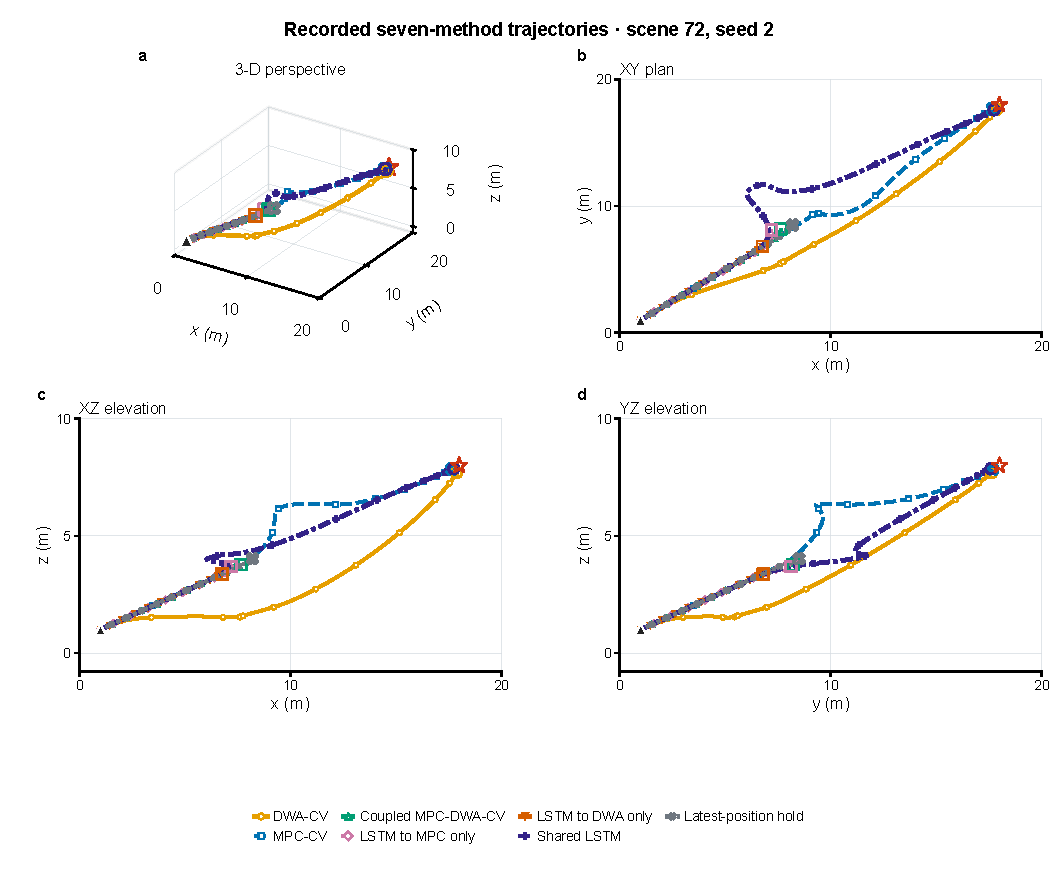
\includegraphics[width=0.98\linewidth]{figures/route_comparison_seven_method_scene72_seed2.pdf}
\caption{Seven-method simulated trajectories from scene 72, seed 2. (a) 3-D perspective; (b) XY plan; (c) XZ elevation; (d) YZ elevation. All six comparator paths span at least 5 s. Shared LSTM and standalone DWA achieved collision-free goal arrival; standalone MPC reached goal tolerance after swept contact; position-hold MPC--DWA collided before arrival; the other three coupled variants stopped without contact. Each route contains only saved positions through its logged terminal state. Color, line style and sparse markers at recorded states identify the method; terminal circles, squares and crosses mark safe arrival, no-contact non-arrival and a run with swept contact, respectively (the cross is not the collision location). This matched case illustrates route geometry; aggregate comparisons use the complete evaluation.}
\label{fig:seven-method-routes}
\end{figure}

\subsection*{S8.2. Seven-method outcomes}
The run-level outcomes, denominators, clustered intervals, paired contrasts, secondary distributions and failure-category counts are archived with the v13 evidence package. These results are presented only after all 2,100 episode keys pass integrity and coverage checks; they are not pooled with the earlier 500-scene benchmark or the 4,320-episode development set.

\needspace{7\baselineskip}
\section*{S9. Reproducibility files}
The reproducibility materials distinguish the 100-scene seven-method exploratory evaluation from the completed historical five-controller benchmark and the separate 4,320-episode Stage-1 development calibration. Scene identifiers, seeds and motion families are recorded in each scenario manifest; their SHA-256 values are listed in the audit records:
\begin{center}
\small\texttt{10D86F1D0BA1146B9777C82A63AFCFB526DA9E309C961D4B5B1A849C4D9BCCF1}
\end{center}
The v13 evidence archive contains the manuscript sources, figures, bilingual reader, historical run-level records, Stage-1 recovered episode table, seven-method exploratory aggregates and their integrity manifests. Original episode MAT checkpoints remain unchanged in the project results directory and are not duplicated in the archive; their SHA-256 hashes are included. The incomplete Stage-2 calibration remains excluded from outcome claims. These experiments use prescribed obstacle tracks; no real-flight result or public data DOI is claimed here.

\begin{table}[H]
\centering
\caption{Artifacts documenting the reported historical benchmark and separate Stage-1 development calibration. The two evidence sets are not pooled.}
\label{tab:repro-index}
\footnotesize
\renewcommand{\arraystretch}{0.95}
\begin{tabularx}{\linewidth}{@{}>{\raggedright\arraybackslash}p{0.37\linewidth}X>{\raggedright\arraybackslash}p{0.19\linewidth}@{}}
\toprule
Artifact & Purpose & Expected content \\
\midrule
\texttt{scenario\_manifest.csv} & Historical assignment of scene identifiers, seeds and motion families & 500 historical scenes \\
\texttt{five\_method\_run\_audit.csv} & Historical run-level joined audit & 7,500 historical rows \\
\texttt{five\_method\_terminal\_outcomes.csv} & Historical mutually exclusive terminal accounting used in Table S7 & 5 controllers; 1,500 each \\
\texttt{five\_method\_summary.csv} & Historical controller-level arrival, collision, clearance and timing summaries & 5 controllers \\
\texttt{five\_method\_paired\_bootstrap.csv} & Historical shared-minus-comparator scene-cluster intervals & 20,000 resamples \\
\texttt{five\_method\_absolute\_bootstrap.csv} & Historical absolute scene-cluster intervals for each controller & 20,000 resamples \\
\texttt{confirmatory\_protocol\_clarification.md} & Historical shared-versus-DWA-only design and stopping rule & 500 scenes; 3 seeds; 1-s DWA \\
\texttt{original\_mpc\_dwa\_baseline\_protocol.md} & Protocol for the historical project-local latest-position reconstruction & 1,500 historical runs \\
\texttt{v12a\_stage1\_recovery\_audit\_20261014.md} & Independent validation and selection record for Stage 1 & 4,320 existing episodes; 0 new simulations \\
\texttt{pooled\_development\_raw.csv} & Stage-1 recovered run-level outcomes & 4,320 rows \\
\texttt{pooled\_episode\_sha256.csv} & Hashes linking the outcomes to preserved MAT checkpoints & 4,320 hashes \\
\texttt{pooled\_calibration\_artifact\_sha256.csv} & Stage-1 calibration artifact integrity register & 8 files \\
\texttt{reproducibility\_package.zip} & Current unified v13 source, data and audit archive & SHA-256 sidecar \\
\texttt{scripts/} & Versioned simulation, recovery and analysis code & Historical and development workflows \\
\bottomrule
\end{tabularx}
\end{table}

\section*{S10. Verified outcomes from the 100-scene exploratory evaluation}
All 2,100 planned episodes passed integrity checks. Table~\ref{tab:v13-seven-method-outcomes} reports collision-free arrivals and swept contacts for seven arms (300 episodes per arm); Table~\ref{tab:v13-seven-method-contrasts} gives the six paired shared-LSTM contrasts.

\begin{table}[H]
\centering
\caption{Observed collision-free goal arrivals and swept contacts in the verified 100-scene exploratory evaluation. Each arm has 300 episodes (100 scenes with three matched seeds).}
\label{tab:v13-seven-method-outcomes}
\footnotesize
\renewcommand{\arraystretch}{1.12}
\setlength{\tabcolsep}{4pt}
\begin{tabularx}{\linewidth}{@{}>{\raggedright\arraybackslash}Xrr@{}}
\toprule
Method & Collision-free arrivals, $n/300$ (\%) & Swept contacts, $n/300$ \\
\midrule
Standalone DWA (CV) & 234/300 (78.0\%) & 0/300 \\
Standalone MPC (CV) & 276/300 (92.0\%) & 15/300 \\
Coupled MPC--DWA (CV in both layers) & 204/300 (68.0\%) & 0/300 \\
MPC--DWA (LSTM to MPC only) & 219/300 (73.0\%) & 0/300 \\
MPC--DWA (LSTM to DWA only) & 224/300 (74.7\%) & 0/300 \\
MPC--DWA (shared LSTM) & 221/300 (73.7\%) & 0/300 \\
Reconstructed MPC--DWA (latest-position hold) & 172/300 (57.3\%) & 50/300 \\
\bottomrule
\end{tabularx}
\end{table}

\needspace{3\baselineskip}
For paired inference, the three seeds were averaged within each scene; 20,000 scene-cluster bootstrap replicates and a centered max-$|t|$ critical value of 2.59005 gave simultaneous 95\% intervals. Differences are in percentage points (pp), with positive values favoring shared LSTM for collision-free arrival.

\begin{table}[H]
\centering
\caption{Shared-LSTM minus comparator differences in collision-free goal-arrival rate. Intervals are simultaneous 95\% scene-cluster bootstrap intervals across the six comparisons.}
\label{tab:v13-seven-method-contrasts}
\footnotesize
\renewcommand{\arraystretch}{1.12}
\setlength{\tabcolsep}{4pt}
\begin{tabularx}{\linewidth}{@{}>{\raggedright\arraybackslash}Xr>{\raggedright\arraybackslash}p{0.34\linewidth}@{}}
\toprule
Comparator & Difference (pp) & Simultaneous 95\% CI (pp) \\
\midrule
Standalone DWA (CV) & $-4.3$ & $[-16.8,\ 8.1]$ \\
Standalone MPC (CV) & $-18.3$ & $[-29.6,\ -7.0]$ \\
Coupled MPC--DWA (CV) & $+5.7$ & $[-3.4,\ 14.7]$ \\
MPC--DWA (LSTM to MPC only) & $+0.7$ & $[-9.0,\ 10.3]$ \\
MPC--DWA (LSTM to DWA only) & $-1.0$ & $[-4.8,\ 2.8]$ \\
Reconstructed MPC--DWA (latest-position hold) & $+16.3$ & $[5.1,\ 27.6]$ \\
\bottomrule
\end{tabularx}
\end{table}

Among the six contrasts, shared LSTM exceeded the latest-position-hold reconstruction, while standalone MPC-CV exceeded shared LSTM; the other four intervals included zero.

Integrity: all 2,100 planned keys appear once. One invalid-sidecar scene-58/seed-2 attempt was preserved but excluded; raw results, logs and hashes remain archived. No planned key fails. Historical 500-scene, 4,320-development, CV/Kalman and scene-404 records remain separate and were not pooled.

\end{document}
